\chapter{Proposed Approach}
Our work builds upon certain aspects of the previous research while introducing a novel and more innovative method for predicting movement origins using machine learning. 
Similar to the previous approach, the pipeline to reach the 20-joints skeleton remains the same (see Sections \ref{sec:orig_markers}, \ref{sec:reduced_markers}).

We chose to utilize an ensamble of some movements from the previous dataset (the one used in \cite{kolykhalova:2020}), enriching the number of samples from other internal resources provided by Casa Paganini \cite{casaPaganini}. 
This choice has been motivated by the necessity to have many short samples that clearly present an origin of movement instead of few samples that are hard to infer in terms of origin of movement, in order to 
reach a high-quality data that can be used in machine learning techniques that will be explained in Section \ref{sec:ml_method}.\\
Since we started from the previous work which was based on game theory and the concept of Shapley values in our approach we considered that there is not a clear contribution in terms of added value derived from nodes cooperation. 
Therefore, we opted for WDC (Weighted Degree Centrality) to determine the perceived origin of the movement for the algorithmic approach.\\
Furthermore for visualization purposes we implemented a method to prevent inconsistent coloring behaviours among clusters over time, by introducing a novel cluster stabilization algorithm. 

\section{Roadmap}
From the starting point of our work \cite{kolykhalova:2020}, we re-implemented, improved and modified it to compare the method for identifying the origin of movement obtained based on graphs with our new machine learning-based approach.
The roadmap of this thesis can be outlined as follows: \\
The dataset was initially acquired through manual annotation of movement origins in numerous MoCap videos. 
The results were validated by achieving consensus among multiple annotators. 
Additionally, markers for videos lacking previous labeling were manually assigned and subsequently compressed into clusters.
The central objectives of this thesis encompass the development of:
\begin{itemize}
    \item \textbf{Cluster Stabilization Algorithm} which ensure that clusters, which represent groups of related markers or joints, maintain their consistency and coherence over time. 
    \item \textbf{Graph-based Procedure} to recognize the Origin of Movement by identifying key nodes that play pivotal roles in the motion analysis using an algorithmic method.
    \item \textbf{Machine Learning Approach} to identify the most promising edge of a the skeletal model by finding patterns in data without an algorithmic approach.
\end{itemize}
Given the multifaceted objectives, two parallel pipelines were developed.\\
The first pipeline included the following steps:
\begin{itemize}
    \item Smoothing the time series of each movement using two classical smoothing algorithms.
    \item Extracting physical measurements from the smoothed data.
    \item Applying cosine similarity to pairs of joints linked by arcs based on a model of physical joints in the human body.
    \item Clustering joints for each frame of the movement.
    \item The primary objective here was the temporal stabilization of cluster color changes.
    \item Formation of a second graph with nodes at cluster borders, connected to other clusters. These nodes are weighted based on their connections and ranked across all frames.
\end{itemize}
The second pipeline involved:
\begin{itemize}
    \item Normalizing the dataset in terms of segment length (Time series Sampling), performer's body structure (Skeleton Barycenter and Joints Distance), and the entire trajectory of the movement.
    \item Extracting a wide range of relevant features from the normalized dataset.
    \item Using these features to train a machine learning model.
    \item Evaluating the model's performance using various metrics.
\end{itemize}
Finally, the results from each pipeline are compared.

\clearpage
\begin{figure}[H]
    \centering
    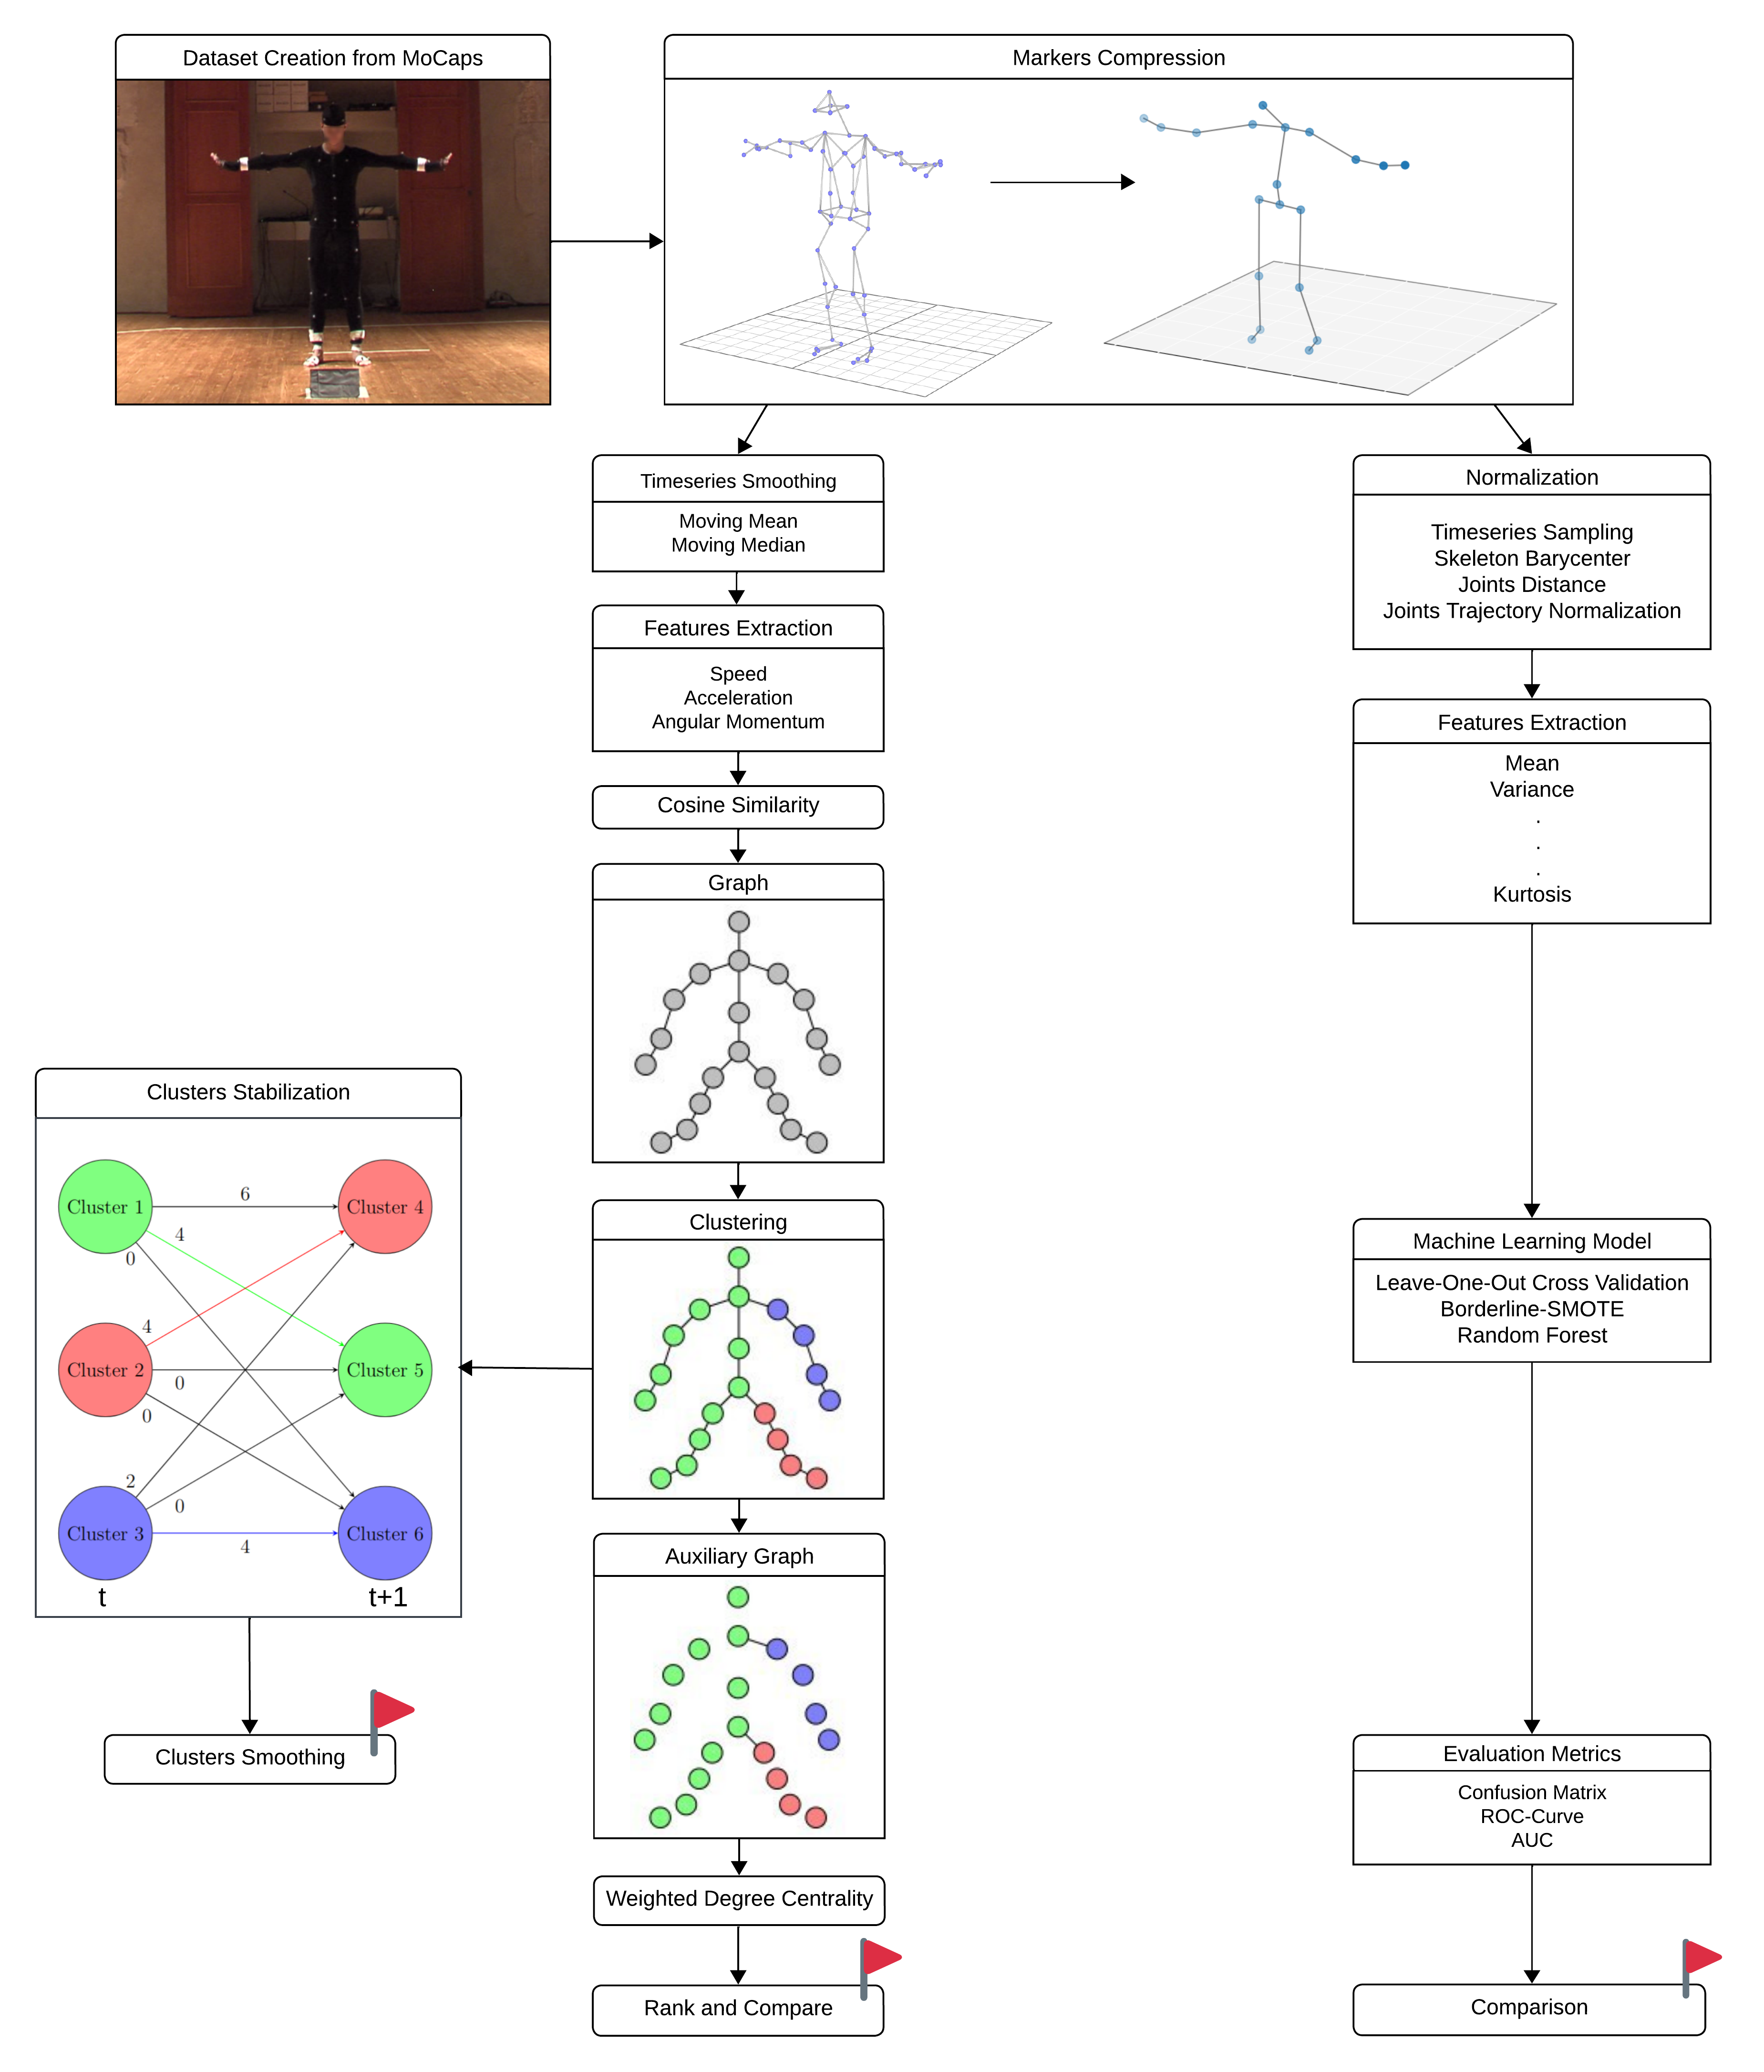
\includegraphics[width=\textwidth,height=\textheight,keepaspectratio]{Walkthrough.png}
    \caption{Roadmap of this Thesis}
    \label{fig:walktrough}
\end{figure}